\documentclass[11pt, a4paper]{article}
\usepackage[UTF8, heading=true]{ctex}
\usepackage[dvipsnames, x11names]{xcolor}
\usepackage{geometry}
\usepackage{subcaption}
\usepackage{float}
\usepackage{graphicx}
\usepackage{listings}

\newfontfamily\codefont{Cascadia Code}
\definecolor{codebackground}{RGB}{230 235 245}

\lstset{
    basicstyle          =   \small\codefont,
    % ---
    tabsize             =   4,
    showstringspaces    =   false,
    numbers             =   left,
    numberstyle         =   \codefont,
    % ---
    breaklines          =   true,
    captionpos          =   t,      
    % ---
    frame               =   l,
    flexiblecolumns,
}

\lstdefinestyle{python}{
    language        =   Python, % 语言选Python
    keywordstyle    =   \bfseries\color{blue},
    % keywordstyle    =   [2] \color{teal},
    stringstyle     =   \color{orange!80!black},
    commentstyle    =   \color{OliveGreen},
    % identifierstyle =   \color{blue!80!white},
    backgroundcolor =   \color{codebackground}
}
\lstMakeShortInline|

\geometry{a4paper, scale=0.8}

\ctexset{
    section = {
        name = {Task },
        format = {\Large\bfseries}
    }
}

\title{\Large{\bf{视听信息系统导论编程3}}}
\author{高艺轩\ 毕嘉仪}
\date{}

\begin{document}
\maketitle
\section{数据准备}
函数|prepare_data|首先将全部文本读入,根据要求进行数据预处理,然后给每一个单独的字符都赋予一个index并将其存储为字典类型,得到对应词表。

\section{完成dataset}

\section{无pos enc、无attn mask的Transformer}
训练结果:\begin{figure}[H]
    \hfill
    \begin{subfigure}[t]{0.45\linewidth}
        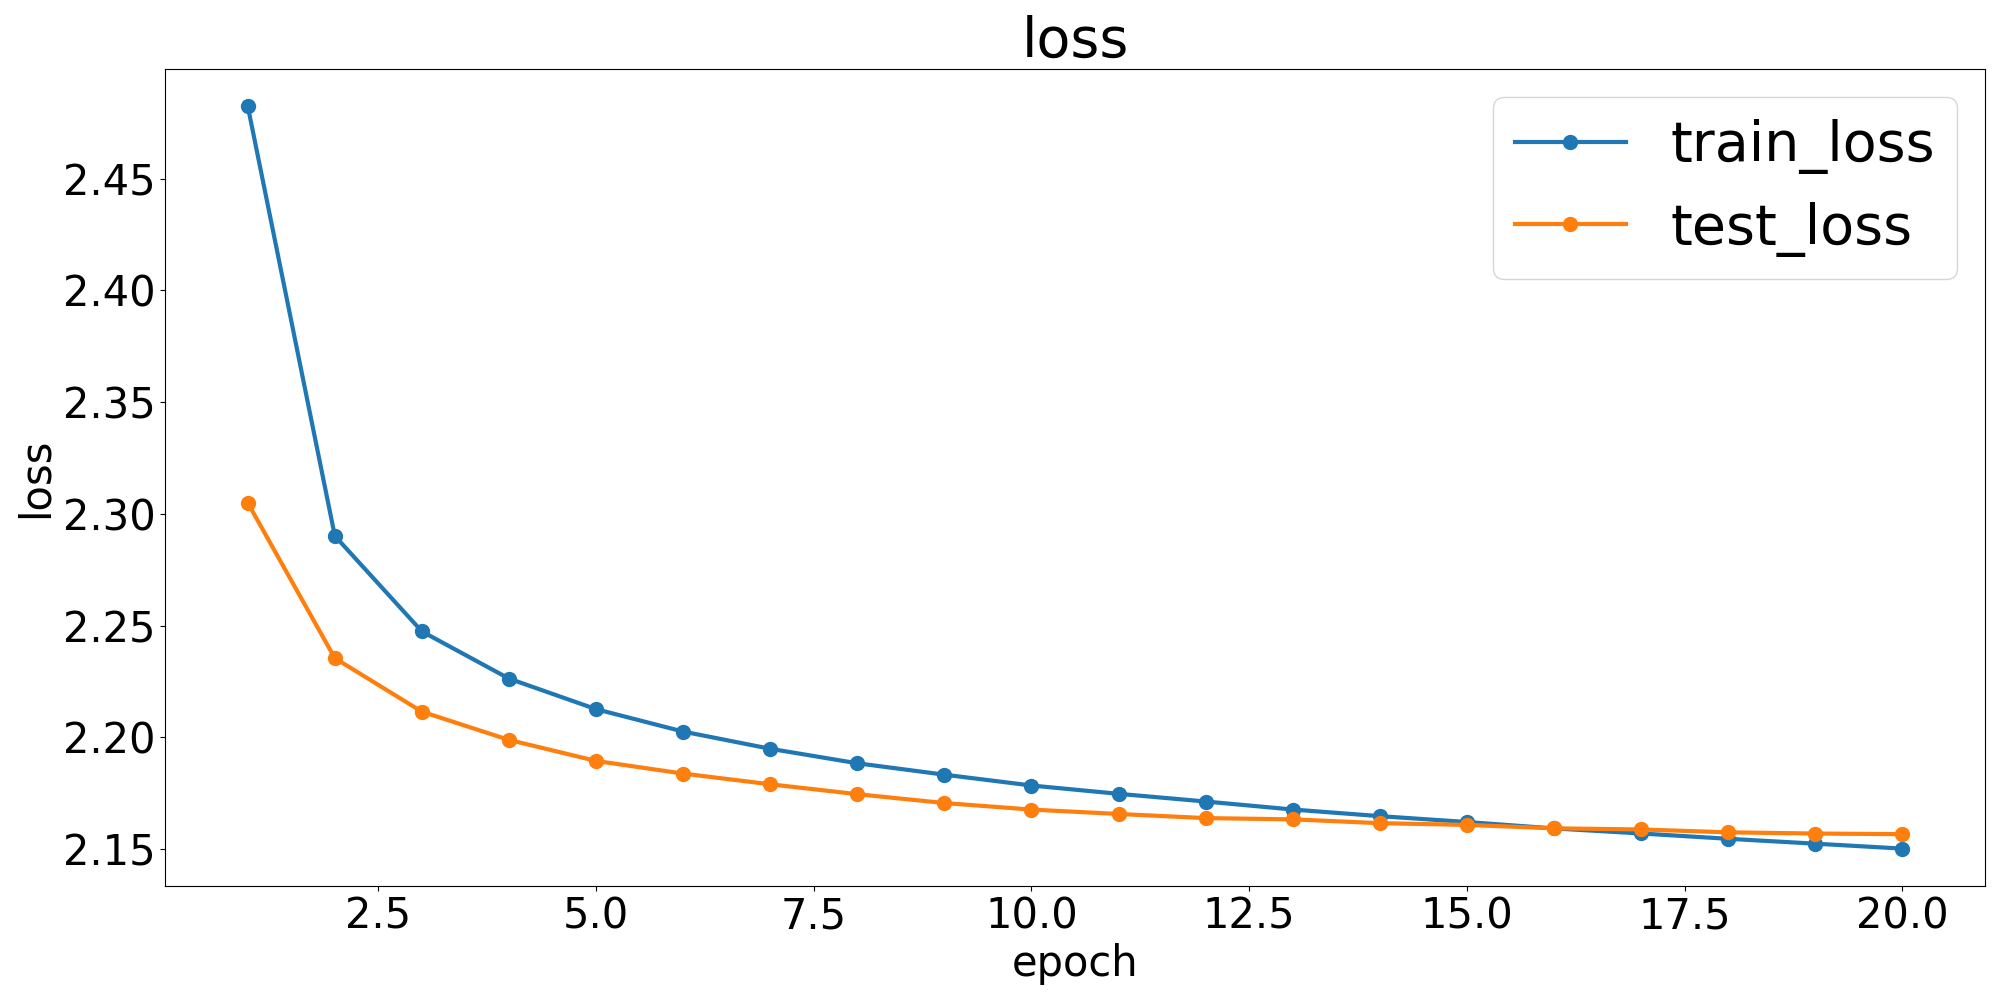
\includegraphics[width=\textwidth]{img/3-1.png}
    \end{subfigure}
    \hfill
    \begin{subfigure}[t]{0.45\linewidth}
        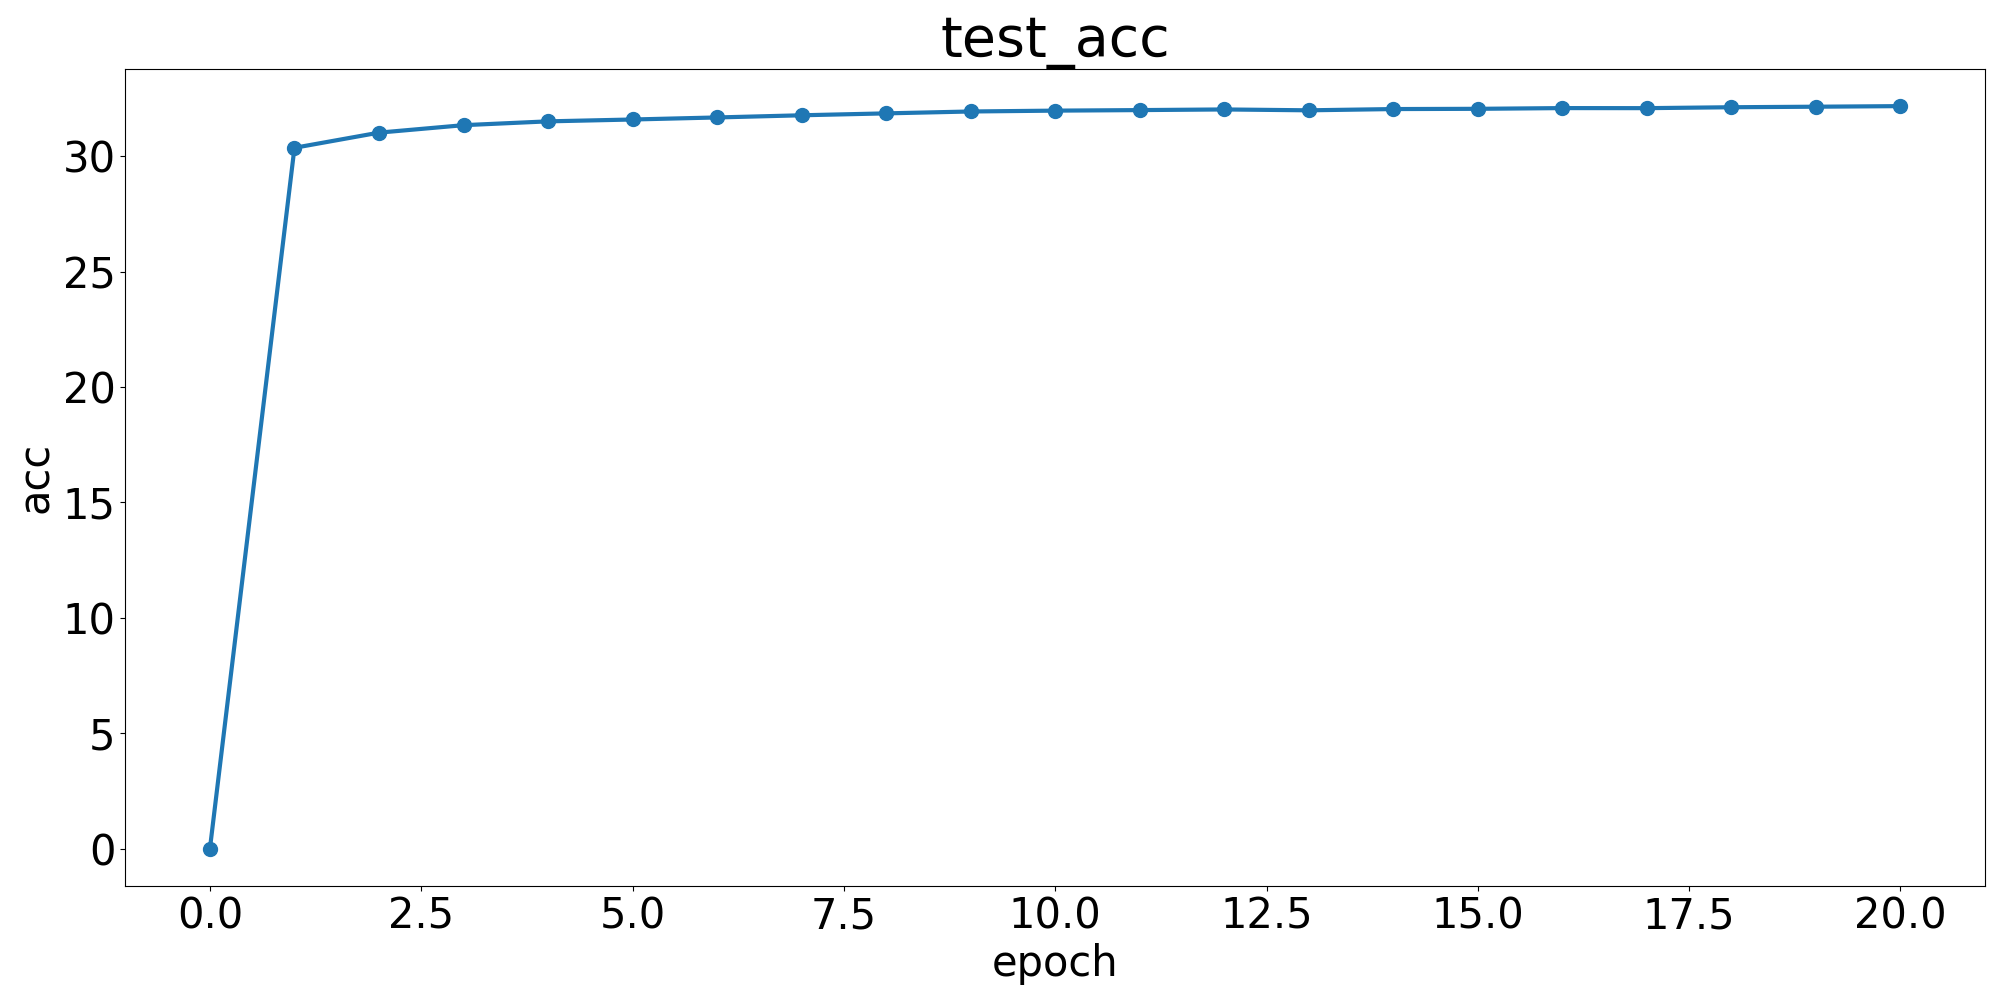
\includegraphics[width=\textwidth]{img/3-2.png}
    \end{subfigure}
    \hfill
\end{figure}


\section{有pos enc、无attn mask的Transformer}
训练结果:
\begin{figure}[H]
    \hfill
    \begin{subfigure}[t]{0.45\linewidth}
        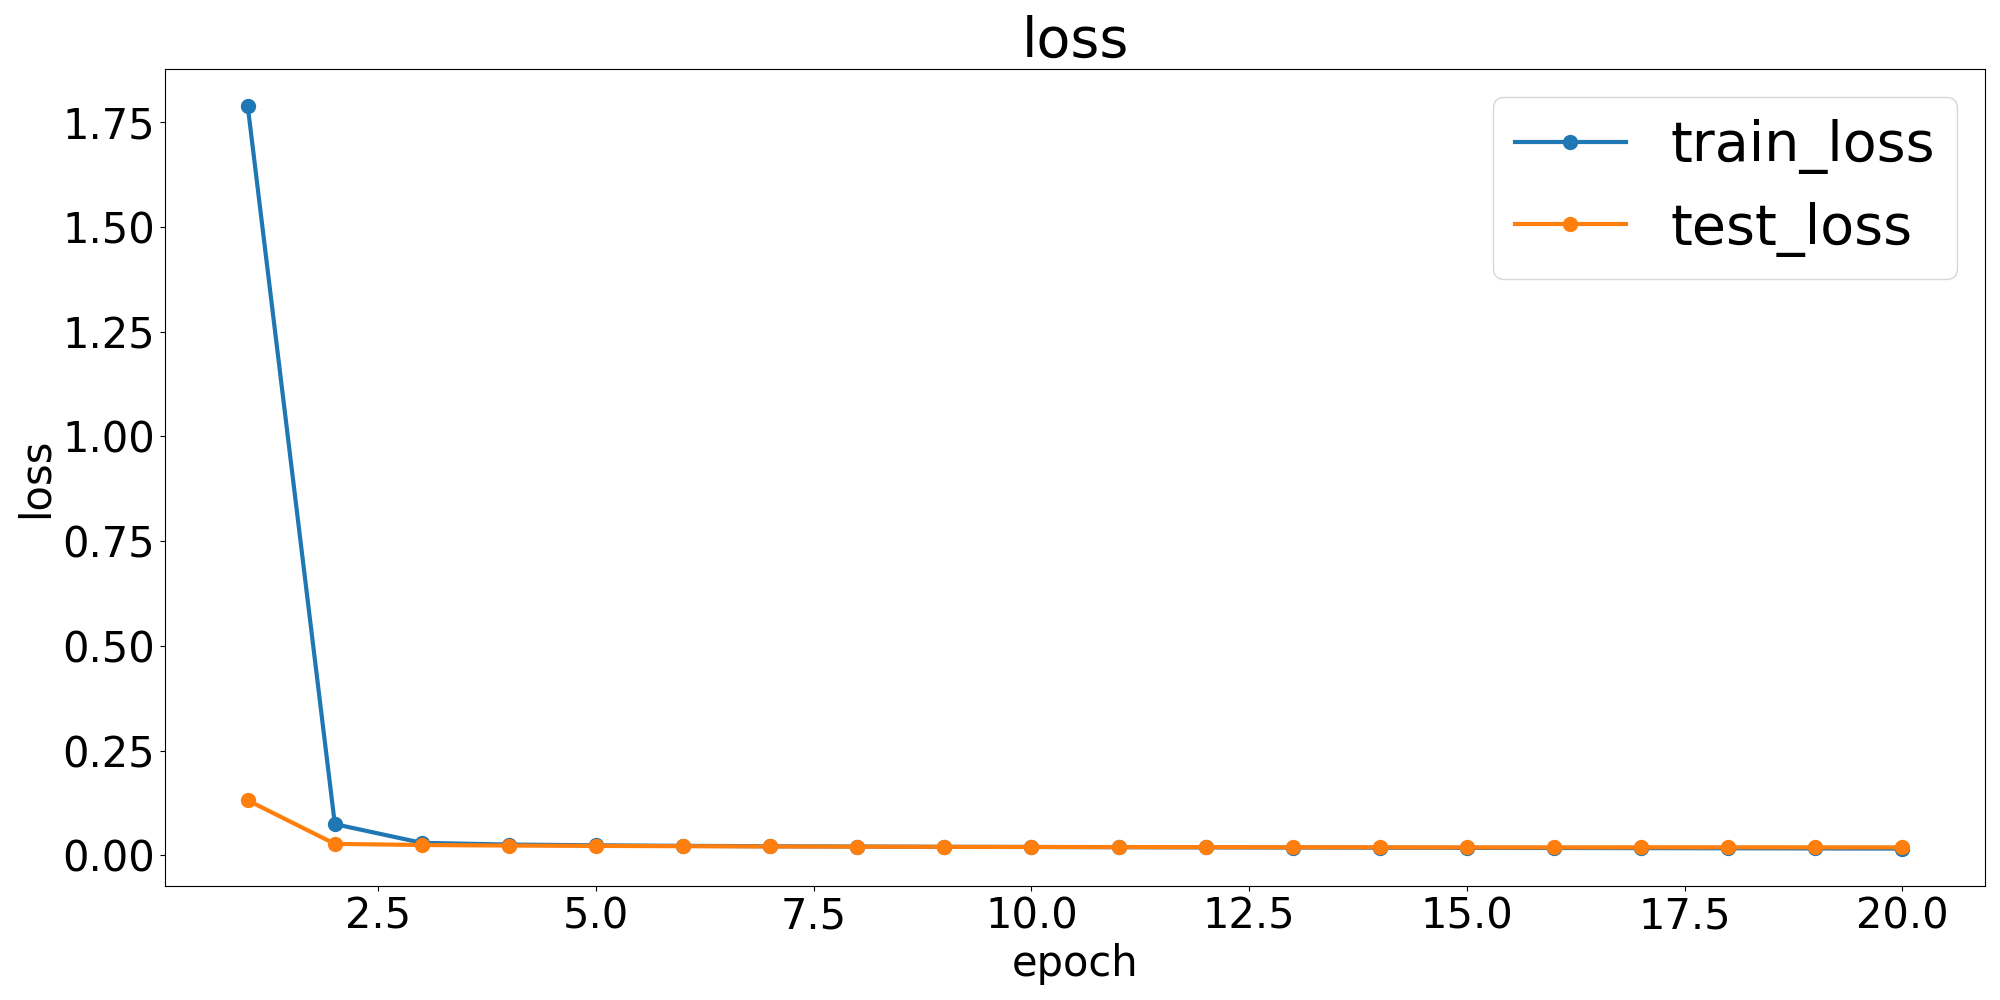
\includegraphics[width=\textwidth]{img/4-1.png}
    \end{subfigure}
    \hfill
    \begin{subfigure}[t]{0.45\linewidth}
        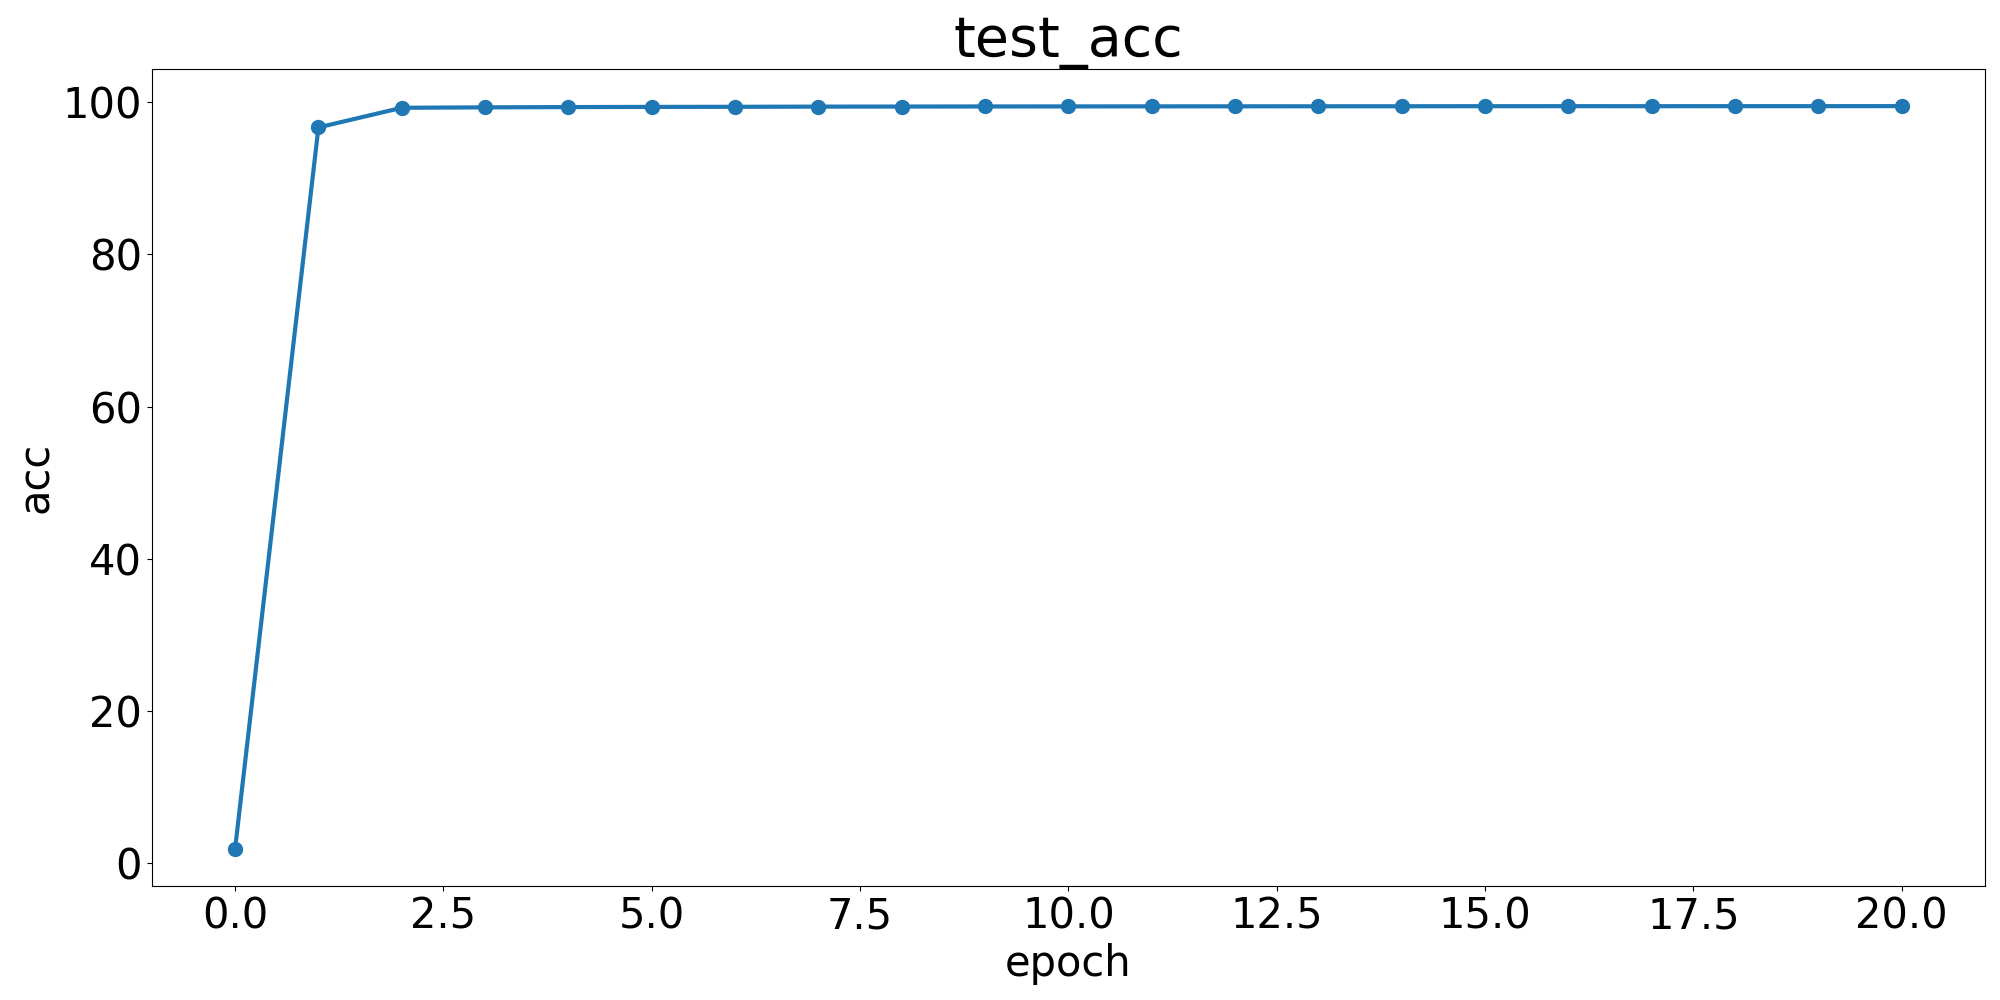
\includegraphics[width=\textwidth]{img/4-2.png}
    \end{subfigure}
    \hfill
\end{figure}


分析positional encoding的作用:

positional encoding通过给每一个词向量添加一部分与位置有关的信息,能够让词向量携带单词在序列中所处位置的信息,从而提高模型对序列的理解能力。


\section{有pos enc、有attn mask的Transformer}
训练结果:
\begin{figure}[H]
    \hfill
    \begin{subfigure}[t]{0.45\linewidth}
        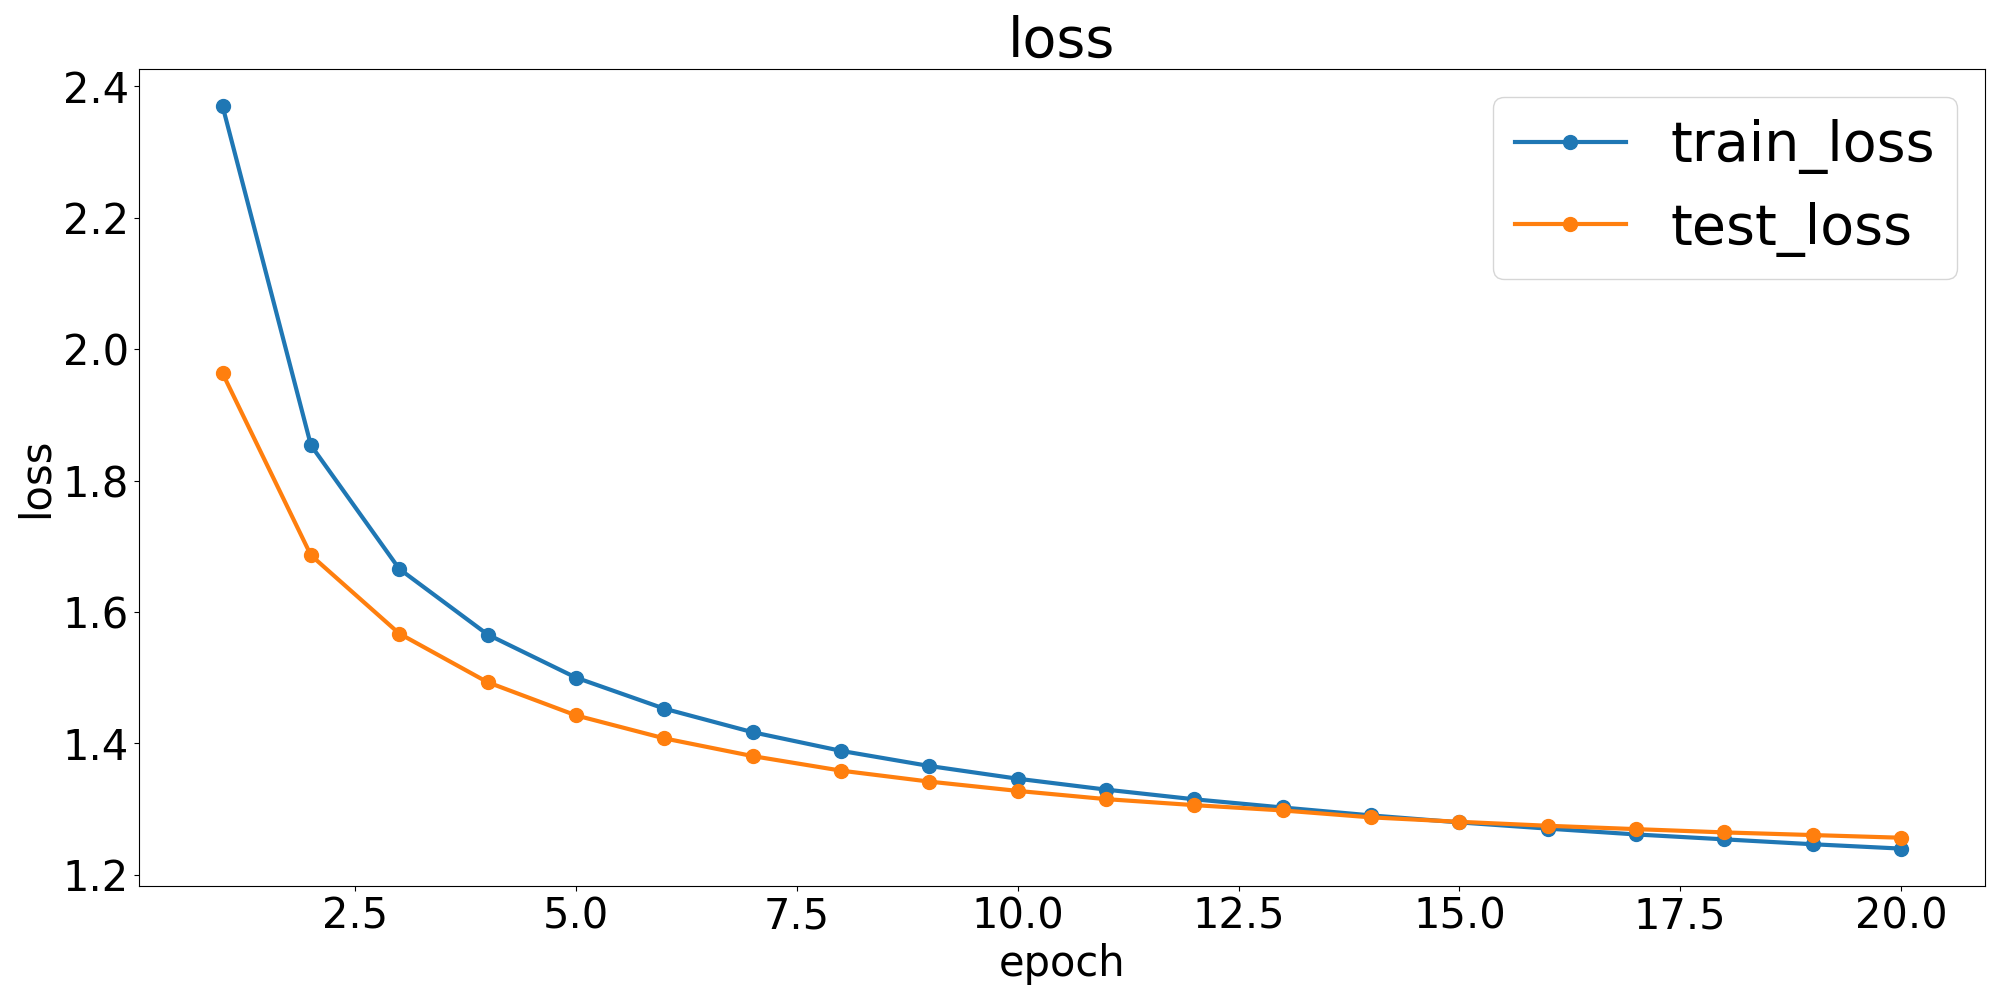
\includegraphics[width=\textwidth]{img/5-1.png}
    \end{subfigure}
    \hfill
    \begin{subfigure}[t]{0.45\linewidth}
        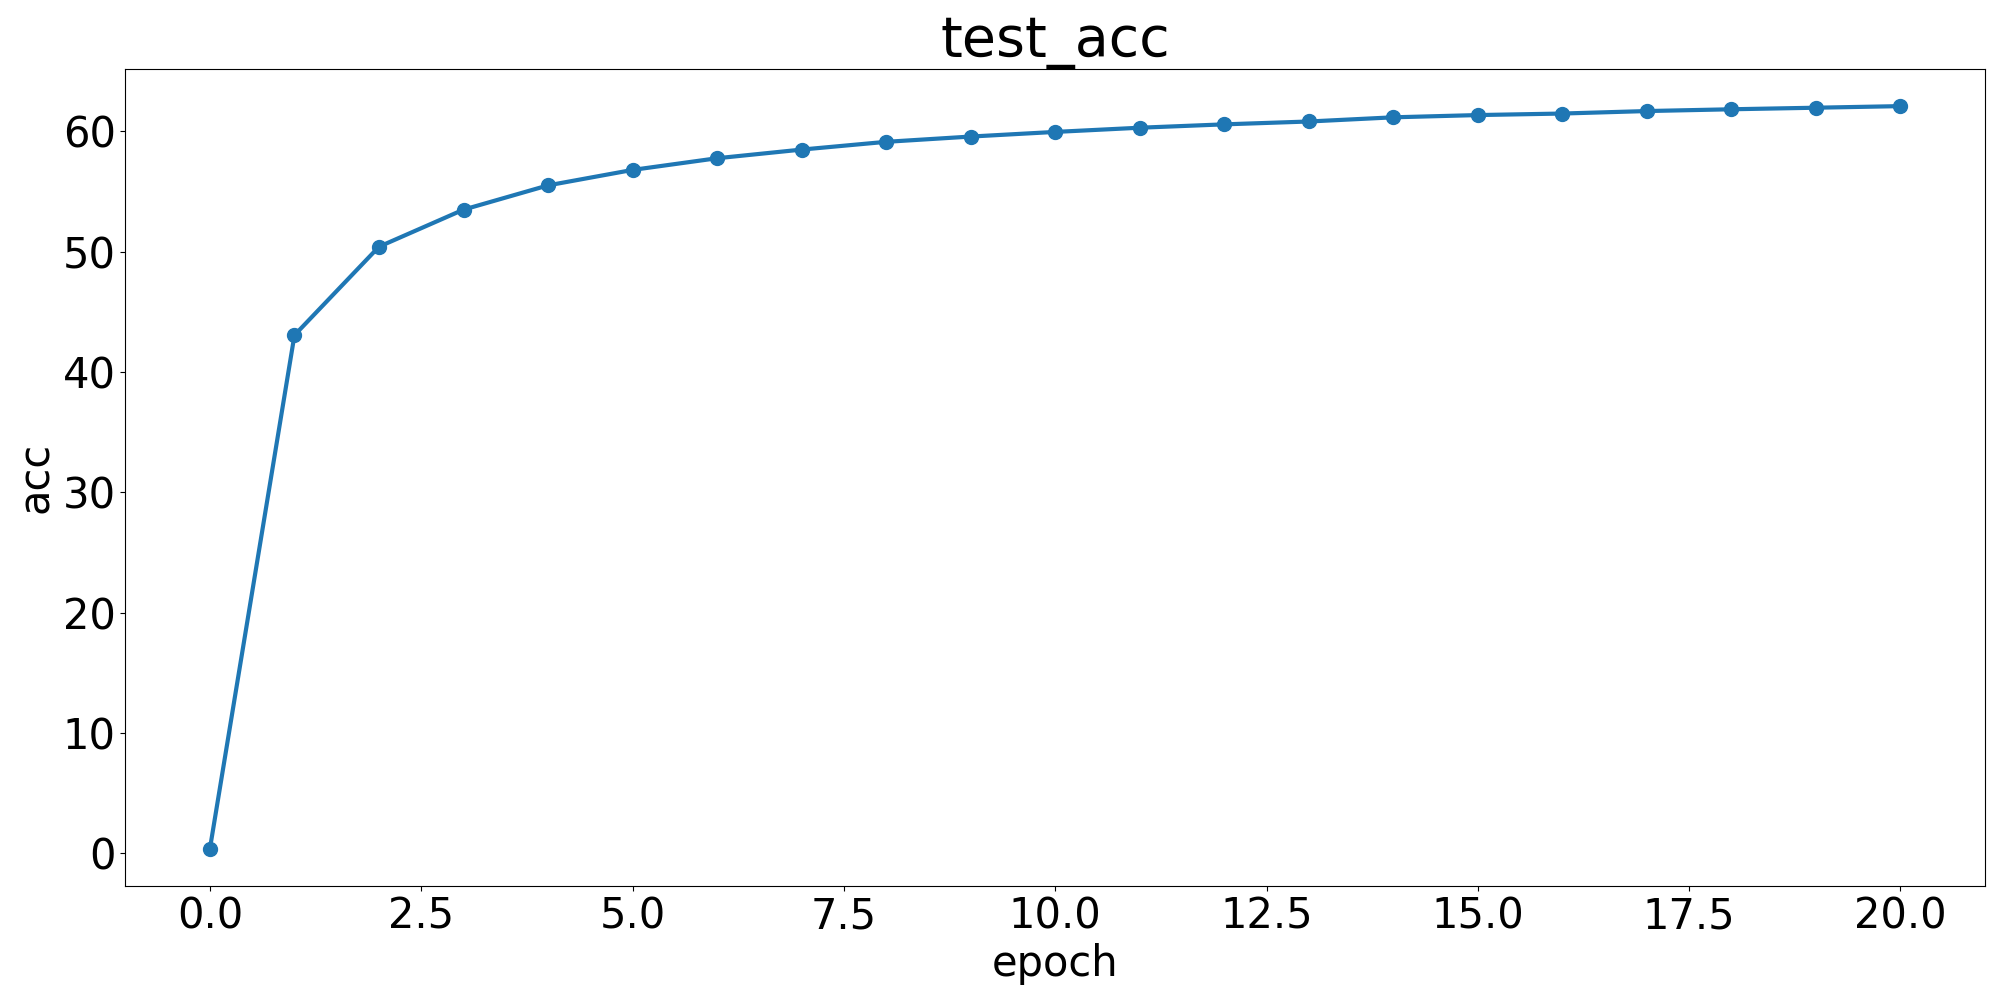
\includegraphics[width=\textwidth]{img/5-2.png}
    \end{subfigure}
    \hfill
\end{figure}


分析attention mask的作用:

attention mask能够确定有效token的位置,即屏蔽掉词向量中不需要模型关注的部分(比如只看当前词语左侧序列,屏蔽右侧序列),从而提高模型的性能和准确性。

\section{默认参数生成}

\section{不同temperature和不同strategy下生成内容的不同}

\section*{程序源代码}
\end{document}